% This is samplepaper.tex, a sample chapter demonstrating the
% LLNCS macro package for Springer Computer Science proceedings;
% Version 2.21 of 2022/01/12
%
\documentclass[runningheads]{llncs}
%
% \usepackage[utf8]{inputenc}
\usepackage[T1]{fontenc}
% T1 fonts will be used to generate the final print and online PDFs,
% so please use T1 fonts in your manuscript whenever possible.
% Other font encondings may result in incorrect characters.


% ---------------------------------------------------------
% Matemáticas
% ---------------------------------------------------------
\usepackage{amsmath,amssymb}
% ---------------------------------------------------------
% Tablas
% ---------------------------------------------------------
\usepackage{booktabs}
% \usepackage[table,xcdraw]{xcolor}
\usepackage{multirow}
\usepackage{tabularx}
\usepackage{longtable}

% ---------------------------------------------------------
% Figuras y gráficos
% ---------------------------------------------------------
\usepackage{graphicx}
\usepackage{subcaption}
\usepackage{float}
\usepackage{pdflscape}
\usepackage{lscape}

% ---------------------------------------------------------
% Algoritmos
% ---------------------------------------------------------
\usepackage{algorithm}
\usepackage{algpseudocode}   % incluye algorithmicx
% ---------------------------------------------------------
% Bibliografía
% ---------------------------------------------------------
% \usepackage[numbers,sort&compress]{natbib} % LNCS ya ahce sort y compress

% ---------------------------------------------------------
% Texto y utilidades
% ---------------------------------------------------------
\usepackage{soul}
\usepackage{seqsplit}
\usepackage{url}
% ---------------------------------------------------------
% TikZ y diagramas
% ---------------------------------------------------------
\usepackage{tikz}
\usetikzlibrary{positioning,arrows.meta}

% ---------------------------------------------------------
% PGFPlots
% ---------------------------------------------------------
\usepackage{pgfplots}
\pgfplotsset{compat=1.18}
\usepackage{pgfplotstable}


% Used for displaying a sample figure. If possible, figure files should
% be included in EPS format.
%
% If you use the hyperref package, please uncomment the following two lines
% to display URLs in blue roman font according to Springer's eBook style:
%\usepackage{color}
%\renewcommand\UrlFont{\color{blue}\rmfamily}
%\urlstyle{rm}
%
\begin{document}
%
\title{On the Impact of Linguistic Granularity and Fuzzy Semantic Design in Particle Swarm Optimization}



%
\titlerunning{On the Impact of Linguistic Granularity and Fuzzy Semantic Design in PSO}
% If the paper title is too long for the running head, you can set
% an abbreviated paper title here
%
\author{
José Barrera-García     \inst{1,2}* \orcidID{0009-0007-9934-5250} \and 
Broderick Crawford      \inst{1}*    \orcidID{0000-0001-5500-0188} \and
Eric Monfroy            \inst{3}    \orcidID{0000-0001-7970-1368} \and 
Felipe Cisternas-Caneo  \inst{1,2}  \orcidID{0000-0001-7723-7012} \and
Ricardo Soto            \inst{1}    \orcidID{0000-0002-5755-6929} \and
Giovanni Giachetti      \inst{4}    \orcidID{0000-0003-2809-5120}
%José Manuel Gomez-Pulido\inst{2}\orcidID{0000-0002-6897-8262} \and
% Alberto Garces-Jimenez \inst{2}\orcidID{0000-0002-1365-9280}
}

%
\authorrunning{J. Barrera-García et al.}
% First names are abbreviated in the running head.
% If there are more than two authors, 'et al.' is used.
%
\institute{Pontificia Universidad Católica de Valparaíso, Chile \\
\email{\{jose.barrera,broderick.crawford, ricardo.soto\}@pucv.cl}\\ 
\email{felipe.cisternas.c@mail.pucv.cl}\\
\and
Universidad de Alcalá, Spain \\
\and
Université d' Angers, LERIA, France \\
\email{eric.monfroy@univ-angers.fr}
\and
Universidad Andres Bello, Chile \\
\email{giovanni.giachetti@unab.cl}
}


%
\maketitle              % typeset the header of the contribution
%
\begin{abstract}
The effectiveness of fuzzy-controlled Particle Swarm Optimization (PSO) largely depends on design choices that are often treated as secondary implementation details. While fuzzy control systems are used to adapt metaheuristic parameters, the impact of linguistic granularity and membership function design is rarely analyzed explicitly. This paper presents a focused experimental study of a swarm-level fuzzy-controlled PSO, providing an initial empirical assessment of three- and five-label linguistic schemes under identical control logic driven by iteration progress and population diversity. Results on representative benchmark functions show that fuzzy control improves robustness and average performance in complex multimodal landscapes, while providing no benefit in unimodal or structurally regular problems. These findings indicate that fuzzy semantic design constitutes a relevant experimental dimension in adaptive metaheuristics and should be analyzed explicitly rather than assumed as fixed.


\keywords{Particle Swarm Optimization \and Fuzzy Control \and Metaheuristics \and Online Parameter Adaptation \and Linguistic Granularity.}


\end{abstract}

%%%%%%%%%%%%%%%%%%%%%%%%%%%%%%%%%%%%%%%
%%%%%%%%%%%%%%% SECTION %%%%%%%%%%%%%%%
%%%%%%%%%%%%%%%%%%%%%%%%%%%%%%%%%%%%%%%
\section{Introduction}

Particle Swarm Optimization (PSO) is a population-based metaheuristic whose performance is strongly influenced by the balance between global exploration and local exploitation \cite{kennedy1995particle}. The inertia weight plays a key role in regulating this balance, motivating numerous adaptive strategies aimed at improving convergence behavior and robustness \cite{shi1998modified}.

Fuzzy control systems have been widely employed to adapt PSO parameters online using qualitative descriptions of the search state, providing a flexible alternative to deterministic or iteration-based schedules \cite{shi2001fuzzy}. However, most fuzzy-controlled PSO variants rely on fixed linguistic partitions and predefined membership functions selected a priori, typically without explicit analysis of their semantic design.

As a result, the impact of linguistic granularity and membership function configuration remains insufficiently explored. In particular, it is unclear to what extent different fuzzy linguistic schemes, even when sharing identical control logic, influence optimization behavior across problems with different landscape characteristics.

This paper presents an experimental analysis of fuzzy-controlled PSO variants that differ exclusively in linguistic granularity and membership function design. Rather than proposing a new optimization algorithm, the study isolates and evaluates the effect of alternative fuzzy semantic configurations under identical control logic, assessing their impact on performance and robustness across representative benchmark functions. The results position fuzzy scheme design as a relevant, yet often overlooked, experimental dimension in adaptive metaheuristic optimization.

The remainder of this paper is organized as follows. Section~\ref{sec:related_work} reviews relevant work on fuzzy-adaptive parameter control in PSO and related optimization frameworks. Section~\ref{sec:fcs_pso} describes the fuzzy-controlled PSO framework and the linguistic configurations evaluated in this study. Section~\ref{sec:experimental_setup} details the benchmark functions, parameter settings, and experimental protocol. The experimental results and their discussion are presented in Section~\ref{sec:results}. Finally, Section~\ref{sec:conclusiones} summarizes the main findings and outlines directions for future research.



%%%%%%%%%%%%%%%%%%%%%%%%%%%%%%%%%%%%%%%%%%%%%%%%%%%%%
%%%%%%%%%%%%%%%%%%%    SECTION     %%%%%%%%%%%%%%%%%%
%%%%%%%%%%%%%%%%%%%%%%%%%%%%%%%%%%%%%%%%%%%%%%%%%%%%%
\section{Related Work}
\label{sec:related_work}

Adaptive parameter control has been extensively investigated as a means to improve the robustness and efficiency of population-based metaheuristics, particularly Particle Swarm Optimization (PSO). Early approaches primarily relied on fixed or iteration-dependent inertia weight schedules; however, such strategies are inherently limited by their inability to react to the evolving state of the swarm and the search landscape.

\vspace{-0.25cm}
\subsection{Fuzzy Logic for Adaptive Parameter Control in PSO} Fuzzy logic was introduced into PSO to enable qualitative, state-dependent adaptation of the inertia weight, overcoming the rigidity of deterministic schedules. The seminal work by Shi and Eberhart proposed a fuzzy system that adjusted inertia based on swarm performance indicators, demonstrating improved adaptability over static and linearly decreasing schemes \cite{shi2001fuzzy}. Subsequent studies extended this approach by incorporating richer sets of swarm-level indicators and more elaborate fuzzy controllers. Comparative analyses reported that fuzzy-adaptive inertia mechanisms outperform classical PSO variants across diverse benchmark functions, particularly when combined with co-evolutionary or hybrid strategies \cite{valdez2017comparative,noronha2021diversity}. More recent contributions have explored advanced fuzzy architectures for PSO parameter adaptation. Nobile et al.\ proposed a fuzzy self-tuning PSO that adjusts multiple parameters at the particle level, yielding competitive or superior performance compared to PSO, DE, and CMA-ES \cite{nobile2018fuzzy}. Similarly, Xia et al.\ introduced a multiple-input multiple-output fuzzy controller for adapting learning weights and elite selection mechanisms, reporting strong performance on large-scale and multimodal benchmarks \cite{xia2022particle}. Structured fuzzy representations, such as fuzzy signatures, have also been investigated to regulate inertia using hierarchical linguistic information \cite{komarudin2021signature}. Beyond fuzzy-based strategies, parameter control and meta-level adaptation have been widely explored in the context of hyperheuristics and adaptive metaheuristics, where control mechanisms are used to regulate algorithmic behavior based on search dynamics \cite{crawford2013parameter,talbi2009metaheuristics}. Recent contributions in the Optimization and Learning community further highlight the relevance of systematic experimental analysis when designing adaptive control mechanisms for metaheuristics \cite{abrego2023multi,cisternas2025objective}.


\vspace{-0.25cm}
\subsection{Membership Function Design and Linguistic Granularity}

Beyond the selection of input variables and control architecture, the design of membership functions and the choice of linguistic granularity have a direct impact on the behavior of fuzzy-adaptive PSO. Comparative studies on interval type-2 fuzzy systems have shown that different membership function shapes can lead to statistically significant performance differences, even when the rule base remains unchanged \cite{olivas2014comparative}. This indicates that membership functions encode semantic information that actively influences control dynamics.

Related evidence from fuzzy control and learning systems reinforces this observation. Metaheuristic-based tuning of membership functions has been shown to improve accuracy and robustness in classical control problems, while alternative bio-inspired optimizers yield comparable gains across real-world applications \cite{fierro2013optimization,nikolic2020bee}. In learning contexts, PSO-assisted neuro-fuzzy models employing enriched linguistic representations demonstrate that semantic expressiveness can enhance performance when appropriately configured \cite{chatterjee2007pso}.

\vspace{-0.25cm}
\subsection{Linguistic Representation and Granular Computing in Optimization}

In parallel with fuzzy-adaptive PSO research, studies on linguistic information granulation have highlighted the influence of linguistic scale design and semantic resolution on optimization and decision-making processes. Linguistic granulation models combined with PSO show that the granularity of linguistic representation affects convergence behavior and solution quality in distributed decision-making settings \cite{huang2022linguistic,zhang2022linguistic}.

Moreover, analyses of multi-granularity linguistic scale consistency indicate that different linguistic resolutions are not neutral transformations. Misaligned linguistic scales can lead to inconsistent aggregation and decision outcomes, underscoring the role of semantic design in systems that rely on linguistic information processing \cite{zhao2021linguistic}.

\vspace{-0.25cm}
\subsection{Positioning of the Present Work}

While existing fuzzy-adaptive PSO approaches typically rely on a single fuzzy configuration fixed throughout the optimization process, the literature provides consistent evidence that both membership function design and linguistic granularity can materially influence optimization performance. However, these semantic design choices are rarely treated as explicit experimental factors in PSO studies.

The present work addresses this gap through a focused experimental analysis of fuzzy-controlled PSO variants that differ exclusively in linguistic granularity and membership function design. Three-label and five-label linguistic schemes are evaluated under consistent control logic and experimental conditions, allowing the isolated assessment of semantic configuration effects. Rather than proposing a new controller architecture, the study aims to empirically characterize how alternative fuzzy semantic representations influence performance and robustness across benchmark problems with distinct landscape characteristics.



%%%%%%%%%%%%%%%%%%%%%%%%%%%%%%%%%%%%%%%%%%%%%%%%%%%%%
%%%%%%%%%%%%%%%%%%%    SECTION     %%%%%%%%%%%%%%%%%%
%%%%%%%%%%%%%%%%%%%%%%%%%%%%%%%%%%%%%%%%%%%%%%%%%%%%%
\section{Fuzzy-Controlled PSO Framework}
\label{sec:fcs_pso}

This section describes the fuzzy-controlled Particle Swarm Optimization (PSO) framework employed in the experimental evaluation. The standard PSO algorithm is extended by incorporating a swarm-level fuzzy control system that dynamically adapts the inertia weight during the optimization process.

\vspace{-0.25cm}
\subsection{Baseline Particle Swarm Optimization}

The baseline corresponds to the canonical PSO formulation, where particle motion is governed by inertia, cognitive attraction toward the personal best, and social attraction toward the global best position. Particle dynamics are defined by
\begin{equation}
    v_i(t+1) = w \cdot v_i(t) + c_1 r_1 \bigl(p_i - x_i(t)\bigr) + c_2 r_2 \bigl(g - x_i(t)\bigr)
    \label{eq:pso_velocity}
\end{equation}
\begin{equation}
    x_i(t+1) = x_i(t) + v_i(t+1)
    \label{eq:pso_position}
\end{equation}
where $p_i$ and $g$ denote the personal and global best positions, and $r_1$, $r_2 \in [0,1]$ are uniformly distributed random variables.

In the baseline configuration, the inertia weight follows a deterministic linear decreasing schedule, ranging from $0.9$ to $0.1$ over the optimization horizon \cite{abualigah2021arithmetic}. This configuration serves as a reference for assessing the effect of fuzzy-controlled inertia adaptation. All remaining PSO parameters are kept identical across experimental configurations to ensure a controlled comparison.



\vspace{-0.25cm}
\subsection{Fuzzy Control System for Inertia Weight Adaptation}

In the fuzzy-controlled variants, a Mamdani-type fuzzy inference system is embedded into the PSO loop and evaluated once per iteration at the swarm level. At iteration $t$, the controller outputs an inertia weight value $w_t$ based on two normalized indicators: iteration progress and population diversity.

Iteration progress is defined as:
\vspace{-0.25cm}
\begin{equation}
    t_{\text{progress}} = \frac{t}{T_{\max}}
    \label{eq:iteration_progress}
\end{equation}
where $T_{\max}$ is the maximum number of iterations. 

Population diversity measures the normalized spatial dispersion of the swarm:
\vspace{-0.25cm}
\begin{equation}
    D(t) = \frac{1}{d} \sum_{k=1}^{d}
    \frac{\max_i x_{i,k}(t) - \min_i x_{i,k}(t)}{U_k - L_k}
    \label{eq:diversity_metric}
\end{equation}
where $d$ is the problem dimensionality and $[L_k, U_k]$ are the bounds of dimension $k$.

The fuzzy controller maps these inputs to an inertia weight constrained to $[w_{\min}, w_{\max}]$. Defuzzification is performed using the centroid method:
\vspace{-0.25cm}
\begin{equation}
    w_t = \frac{\int z \, \mu_{\text{agg}}(z)\, dz}{\int \mu_{\text{agg}}(z)\, dz}
    \label{eq:defuzzification}
\end{equation}
where $\mu_{\text{agg}}(z)$ denotes the aggregated output membership function.

Figure~\ref{fig:fcs_architecture} illustrates the integration of the fuzzy controller within the PSO iteration loop.

% \begin{figure}[ht]
    \centering
    \resizebox{0.75\columnwidth}{!}{
        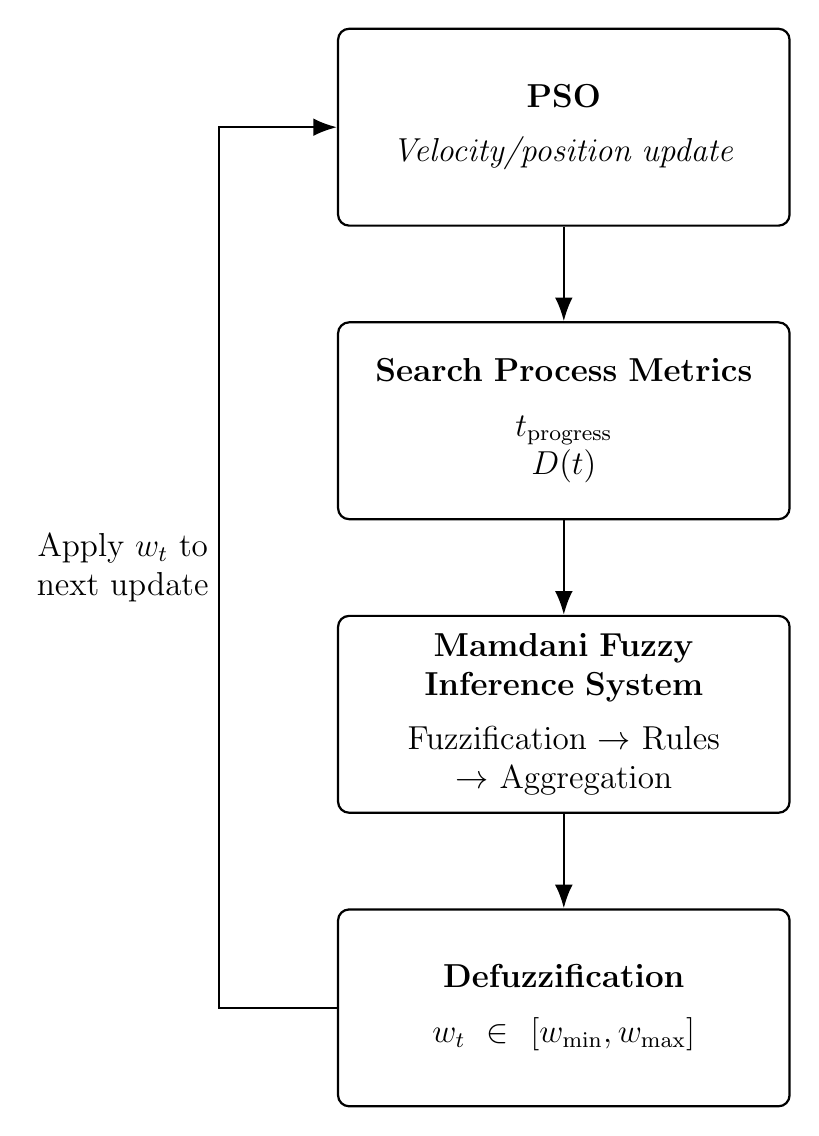
\begin{tikzpicture}[
            font=\large,
            block/.style={
                draw,
                rounded corners,
                align=center,
                minimum height=25mm,
                text width=55mm,
                thick
            },
            arrow/.style={-{Latex[length=3mm]}, thick},
            node distance=12mm
        ]
        
        % Definición de nodos en el eje vertical
        \node[block] (pso) {
            \textbf{PSO}\\
            \vspace{2mm}
            \emph{Velocity/position update}
        };
        
        \node[block, below=of pso] (metrics) {
            \textbf{Search Process Metrics}\\
            \vspace{2mm}
            $t_{\text{progress}}$ \\
            $D(t)$
        };
        
        \node[block, below=of metrics] (fis) {
            \textbf{Mamdani Fuzzy}\\
            \textbf{Inference System}\\
            \vspace{2mm}
            Fuzzification $\rightarrow$ Rules \\
            $\rightarrow$ Aggregation
        };
        
        \node[block, below=of fis] (wt) {
            \textbf{Defuzzification}\\
            \vspace{2mm}
            $w_t \in [w_{\min}, w_{\max}]$
        };
        % Main flow (descending)
        \draw[arrow] (pso) -- (metrics);
        \draw[arrow] (metrics) -- (fis);
        \draw[arrow] (fis) -- (wt);
        
        % Feedback loop
        \draw[arrow] (wt.west) -- ++(-15mm,0) |- 
            node[pos=0.25, left, align=center] {Apply $w_t$ to\\next update} 
            (pso.west);
        
        \end{tikzpicture}
    }
    \caption{Architecture of the Fuzzy-Controlled PSO Framework}
    \label{fig:fcs_architecture_vertical}
\end{figure}
\vspace{-0.5cm}
\begin{figure}[H]
    \centering
    \includegraphics[width=0.9\linewidth]{figures/fcs_architecture.JPG}
    \caption{Architecture of the fuzzy-controlled PSO framework.}
    \label{fig:fcs_architecture}
\end{figure}

\vspace{-1.25cm}
\subsection{Linguistic Schemes and Membership Function Configuration}

Two linguistic granularities are considered: three-label and five-label fuzzy partitions, providing alternative semantic resolutions over identical input and output domains. For each granularity, two predefined configurations (Set~A and Set~B) are evaluated.

Sets~A and~B differ exclusively in membership function shape, overlap, and placement, while preserving identical linguistic variables, universes of discourse, and rule base structure. All membership functions remain fixed throughout the optimization process. This design isolates the effect of semantic resolution from changes in control logic.
% \vspace{-0.5em}

Figure~\ref{fig:membership_comparison_all} depict the membership functions associated with the input variables and the inertia weight output, respectively.
\vspace{-2.5em}

\begin{figure}[H]
    \centering

    % Primera fila
    \subfloat[Diversity membership functions.]{
        
\includegraphics[width=0.45\linewidth]{figures/06_input_diversity_comparison_membership_functions.png}
        \label{fig:diversity_comparison_membership_functions}
    }
    \hfill
    \subfloat[Progress membership functions.]{
        
\includegraphics[width=0.45\linewidth]{figures/06_input_progress_comparison_membership_functions.png}
        \label{fig:progress_comparison_membership_functions}
    }

    % Segunda fila
    %\\
    % \vspace{0.5em}

    \subfloat[Inertia weight membership functions.]{
        
\includegraphics[width=0.7\linewidth]{figures/06_output_w_comparison_membership_functions.png}
        \label{fig:output_membership_comparison}
    }

    \caption{Comparison of input and output membership functions for Sets~A and~B.}
    \label{fig:membership_comparison_all}
\end{figure}


\subsection{Fuzzy Rule Base Configuration}

The fuzzy rule base defines the qualitative mapping between iteration progress, population diversity, and inertia weight. For both linguistic granularities, the same control logic and rule semantics are preserved; differences arise solely from the number of linguistic labels.

To provide a compact representation, the rule bases are visualized using two-dimensional heatmaps that summarize the dominant output linguistic term associated with each combination of input labels.

Figure~\ref{fig:rule_base_comparison} shows that increasing linguistic granularity refines the semantic resolution of the control surface while preserving the underlying control strategy.

\begin{figure}[H]
    \centering
    \subfloat[Fuzzy Rules Base - 3 Labels]{
    
\includegraphics[width=0.49\textwidth]{figures/04_fuzzy_rules_heatmap_3labels.png}
    \label{fig:fuzzy_rules_heatmap_3labels}
    }
    \subfloat[Fuzzy Rules Base - 5 Labels]{
    
\includegraphics[width=0.49\textwidth]{figures/04_fuzzy_rules_heatmap_5labels.png}
    \label{fig:fuzzy_rules_heatmap_5labels}
    }
    \caption{Fuzzy Rules Comparison}
    \label{fig:rule_base_comparison}
\end{figure}





%%%%%%%%%%%%%%%%%%%%%%%%%%%%%%%%%%%%%%%%%%%%%%%%%%%%%
%%%%%%%%%%%%%%%%%%%    SECTION     %%%%%%%%%%%%%%%%%%
%%%%%%%%%%%%%%%%%%%%%%%%%%%%%%%%%%%%%%%%%%%%%%%%%%%%%
\section{Experimental Setup}
\label{sec:experimental_setup}

\subsection{Benchmark Functions}
\label{subsec:benchmarks}

The experimental evaluation was conducted using a reduced set of classical benchmark functions commonly employed in the optimization literature. The selected functions represent optimization landscapes with contrasting characteristics, including unimodal, structurally regular problems in high-dimensional spaces and highly multimodal, rugged landscapes in lower-dimensional domains.

The Sphere function (F1) was used as a unimodal benchmark with a smooth convex landscape and a single global optimum at the origin. In this study, F1 was evaluated in a high-dimensional setting ($d = 100$) to analyze convergence behavior under a large search space. The Griewank function (F11) was considered as a multimodal benchmark in the same dimensionality ($d = 100$), featuring regularly distributed local minima and moderate landscape complexity.

To assess performance under more challenging multimodal conditions, two variants of the Shekel function were selected: configurations with five components (F21) and ten components (F23). These functions are defined in a four-dimensional search space and are characterized by rugged landscapes with multiple deep local minima.

All benchmark functions were implemented using their standard definitions provided by the \texttt{Opfunu} library, ensuring reproducibility and consistency across experiments \cite{abualigah2021arithmetic,Van_Thieu_2024_Opfunu}. Table~\ref{tab:benchmark_functions} summarizes the main characteristics of the selected benchmarks.

\vspace{-0.25cm}


\begin{table}[H]
    \centering
    \begin{tabular}{lccc}
    \toprule
    Function & Type & Dim. & Global Optimum \\
    \midrule
    F1 (Sphere)        & Unimodal   & $100$ & $0.0$ \\
    F11 (Griewank)     & Multimodal & $100$ & $0.0$ \\
    F21 (Shekel, $m=5$)  & Multimodal & $4$   & $-10.1532$ \\
    F23 (Shekel, $m=10$) & Multimodal & $4$   & $-10.5363$ \\
    \bottomrule
    \end{tabular}
    \caption{Benchmark functions used in the experimental evaluation.}
    \label{tab:benchmark_functions}
\end{table}


\vspace{-1cm}

\subsection{Parameter Settings and Evaluation Protocol}
\label{subsec:protocol}

All algorithmic variants were evaluated under identical experimental conditions to ensure a fair comparison. The population size was fixed to $50$ particles and the maximum number of iterations was set to $500$. No additional stopping criteria were applied.

Each algorithm--function combination was executed over $31$ independent runs. To control stochastic variability while preserving comparability, a shared seeding strategy was adopted: all algorithms used the same random seed for the first run, the same (but different) seed for the second run, and so on. The initial seed value was set to $42$ and incremented by one for each subsequent run.

The baseline PSO algorithm was evaluated alongside its fuzzy-controlled variants (PSO--FCS). Four fuzzy configurations were considered, combining two membership function sets (A and B) with two levels of linguistic granularity (three and five labels), denoted as PSO--FCS--A3, PSO--FCS--B3, PSO--FCS--A5, and PSO--FCS--B5. Apart from inertia weight adaptation, all remaining PSO parameters and update equations were kept identical across variants.

Performance was assessed using the final best fitness value obtained at the end of each run and the relative gap to the known global optimum, defined as

\begin{equation}
    \text{Gap}(\%) =
    \frac{\left| f_{\text{best}} - f_{\text{opt}} \right|}
    {\left| f_{\text{opt}} \right|} \times 100
    \label{eq:gap_metric}
\end{equation}

Robustness was evaluated by reporting the mean and standard deviation of the final fitness values across the 31 runs. Computational cost was measured using wall-clock execution time under identical hardware conditions.

All experiments were conducted on a 64-bit system equipped with an Intel Core i7 CPU (2.8~GHz) and 16~GB of RAM. The algorithms were implemented in Python~3.11.9 and executed sequentially on CPU cores only.





%%%%%%%%%%%%%%%%%%%%%%%%%%%%%%%%%%%%%%%%%%%%%%%%%%%%%
%%%%%%%%%%%%%%%%%%%    SECTION     %%%%%%%%%%%%%%%%%%
%%%%%%%%%%%%%%%%%%%%%%%%%%%%%%%%%%%%%%%%%%%%%%%%%%%%%
\section{Results and Discussion}
\label{sec:results}

This section presents the experimental results obtained for the proposed fuzzy-controlled PSO framework and discusses the observed performance patterns across benchmark functions and fuzzy configurations. The analysis focuses on three main aspects: overall performance with respect to standard PSO, the influence of linguistic granularity and fuzzy set design, and the stability of the optimization process across independent runs.

\vspace{-0.25cm}
\subsection{Overall Performance Comparison}
\label{subsec:overall_results}

Table~\ref{tab:performance_summary} presents the comparative performance of standard PSO and fuzzy-controlled PSO variants across the selected benchmark functions. The results clearly indicate that the effectiveness of fuzzy-based inertia weight adaptation is strongly dependent on the characteristics of the optimization landscape, with neither approach uniformly dominating the other.

\vspace{-0.25cm}
\begin{table}[H]
\centering
\small
\resizebox{\textwidth}{!}{%
\begin{tabular}{@{}llcccc@{}}
    \toprule
    \multicolumn{1}{c}{Function} & \multicolumn{1}{c}{Method} & Mean   Fitness & Std.   Dev. & Mean   Gap (\%) & Mean   Execution Time \\ \midrule
    F1  & PSO          & 23.070    & 11.474   & 23.1\%    & 9.903  \\
    F1  & PSO\_FCS:A:3 & 74972.756 & 3560.587 & 74972.8\% & 12.028 \\
    F1  & PSO\_FCS:A:5 & 74768.800 & 3863.507 & 74768.8\% & 12.059 \\
    F1  & PSO\_FCS:B:3 & 74912.469 & 3653.264 & 74912.5\% & 12.076 \\
    F1  & PSO\_FCS:B:5 & 76414.155 & 3178.414 & 76414.2\% & 12.769 \\
    F11 & PSO          & 1.208     & 0.103    & 1.2\%     & 10.308 \\
    F11 & PSO\_FCS:A:3 & 675.755   & 32.045   & 675.8\%   & 12.686 \\
    F11 & PSO\_FCS:A:5 & 674.625   & 34.755   & 674.6\%   & 12.072 \\
    F11 & PSO\_FCS:B:3 & 675.212   & 32.879   & 675.2\%   & 12.176 \\
    F11 & PSO\_FCS:B:5 & 688.725   & 28.603   & 688.7\%   & 12.019 \\ 
    F21 & PSO          & -6.289    & 3.803    & 38.1\%    & 5.928  \\
    F21 & PSO\_FCS:A:3 & -7.649    & 1.598    & 24.7\%    & 6.190  \\
    F21 & PSO\_FCS:A:5 & -7.749    & 1.275    & 23.7\%    & 6.385  \\
    F21 & PSO\_FCS:B:3 & -7.683    & 1.659    & 24.3\%    & 6.216  \\
    F21 & PSO\_FCS:B:5 & -7.699    & 1.602    & 24.2\%    & 6.353  \\
    F23 & PSO          & -7.519    & 3.877    & 28.6\%    & 10.761 \\
    F23 & PSO\_FCS:A:3 & -8.203    & 1.419    & 22.1\%    & 10.973 \\
    F23 & PSO\_FCS:A:5 & -8.133    & 1.279    & 22.8\%    & 11.145 \\
    F23 & PSO\_FCS:B:3 & -8.139    & 1.243    & 22.8\%    & 10.979 \\
    F23 & PSO\_FCS:B:5 & -8.124    & 1.339    & 22.9\%    & 11.133 \\
    \bottomrule
\end{tabular}%
}
\caption{Summary of performance for PSO and fuzzy-controlled variants.}
\label{tab:performance_summary}
\end{table}


\vspace{-1.0cm}


For the unimodal Sphere function (F1) and the structurally regular Griewank function (F11), standard PSO consistently outperforms all fuzzy-controlled variants. In both cases, PSO achieves lower fitness values, reduced variability across runs, and shorter execution times. These results indicate that, in smooth or regularly structured high-dimensional landscapes, adaptive inertia modulation is unnecessary and may interfere with otherwise effective baseline dynamics.

In contrast, for the multimodal Shekel functions (F21 and F23), all fuzzy-controlled variants outperform standard PSO in terms of mean fitness and relative gap. These improvements are accompanied by a marked reduction in standard deviation, indicating enhanced robustness and reduced sensitivity to local optima. Although execution times increase moderately due to fuzzy inference, this overhead remains limited and does not explain the observed performance gains.

Overall, the results show that fuzzy-controlled inertia adaptation is strongly problem-dependent: it degrades performance in unimodal or regular landscapes but provides clear benefits in complex multimodal scenarios by improving stability and convergence reliability.


\vspace{-0.25cm}
\subsection{Effect of Linguistic Granularity and Fuzzy Set Design}
\label{subsec:granularity}

This analysis shows that the impact of linguistic granularity and fuzzy set design is problem-dependent and secondary with respect to landscape characteristics.

For the unimodal Sphere function (F1) and the regular Griewank function (F11), variations in linguistic granularity do not produce meaningful performance differences. All fuzzy-controlled configurations perform worse than standard PSO, regardless of the number of linguistic labels or the selected fuzzy set, indicating that increased semantic resolution cannot compensate for an unsuitable control mechanism.

In contrast, for the multimodal Shekel functions (F21 and F23), differences between three-label and five-label schemes become observable, although they remain moderate. Five-label configurations tend to achieve slightly lower mean gap values and, in some cases, reduced variability, suggesting finer sensitivity in inertia weight adaptation. However, these improvements are incremental and do not establish consistent dominance of higher linguistic granularity.

Regarding fuzzy set design, Sets~A and~B exhibit comparable performance across all functions, with no systematic advantage observed for either configuration.




%%%%%%%%%%%%%%%%%%%%%%%%%%%%%%%%%%%%%%%%%%%%%%%%%%%%%
%%%%%%%%%%%%%%%%%%%    SECTION     %%%%%%%%%%%%%%%%%%
%%%%%%%%%%%%%%%%%%%%%%%%%%%%%%%%%%%%%%%%%%%%%%%%%%%%%
\section{Conclusions and Future Work}
\label{sec:conclusiones}

This paper presented an experimental study of a fuzzy-controlled Particle Swarm Optimization framework, examining whether the semantic design of a fuzzy controller—specifically linguistic granularity and membership function configuration—materially influences inertia weight adaptation and PSO behavior. Rather than proposing a new optimization algorithm, the study empirically evaluated this hypothesis across optimization problems with different structural properties.

The results show that fuzzy-controlled inertia adaptation is not universally advantageous. Standard PSO consistently outperforms fuzzy-controlled variants on unimodal and structurally regular problems, where adaptive modulation of inertia is unnecessary and may disrupt efficient baseline dynamics. In contrast, for complex multimodal problems, fuzzy-controlled PSO achieves improved average performance and enhanced robustness, reflected by lower mean gap values and reduced variability across runs.

Regarding semantic design, linguistic granularity and membership function configuration exhibit a measurable but secondary effect. Increasing the number of linguistic labels can yield modest stability improvements when fuzzy control is effective; however, no single configuration consistently dominates across problems. These observations indicate that the primary source of performance gains lies in the presence of an adaptive control mechanism itself, while semantic refinement acts as a secondary, problem-dependent factor.

Future work will focus on further improving fuzzy control strategies for parameter adaptation in metaheuristics, particularly for complex and highly multimodal problems. Planned extensions include the incorporation of additional search process metrics and the development of dynamic mechanisms capable of selecting or adapting fuzzy control configurations online. In this context, advances at the intersection of machine learning and metaheuristics provide a relevant conceptual foundation for enhancing adaptive control at the meta-level \cite{karimi2022machine}, enabling more flexible and context-aware fuzzy-controlled optimization strategies.









\vspace{-0.25cm}

\section*{Acknowledgements}
\vspace{-0.25cm}
Felipe Cisternas-Caneo was supported by the National Agency for Research and Development ANID BECAS/DOCTORADO NACIONAL 21230203.
José Barrera-García was supported by the National Agency for Research and Development ANID BECAS/DOCTORADO NACIONAL 21242516.

\vspace{-0.25cm}
%
% ---- Bibliography ----
%
% BibTeX users should specify bibliography style 'splncs04'.
% References will then be sorted and formatted in the correct style.
%
\bibliographystyle{splncs04}
\bibliography{bibliography}

\end{document}
